\section{Experiments}~\label{experiment}
% 이 부분도 조금 수정할거야. 0.8을 appx에서 하자고 했는데 이게 아니라 여기서 소개할 게. 그러니까 실험이 2개인 거지, 1. tau에 따른 성능 평가 2. all, no, random, ours에 따른 성능 평가. 

We evaluate the proposed system through two system-level experiments. First, we analyze how the confidence threshold $\tau$ affects task success, execution length, and query frequency. This experiment characterizes the trade-off between autonomous execution and human intervention. Second, we compare four query policies: \textbf{All}, \textbf{No}, \textbf{Random}, and \textbf{Ours}. If a query is triggered, we assume that the human provides the correct answer, which isolates the effect of the query policy from user response errors. A separate user study is then used to examine the user-facing effects of these interaction policies.

\begin{figure}[t!]
    %\captionsetup{skip=0pt} % \hspace{0.3cm}
    \begin{center}
  
    \begin{subfigure}[b]{0.47\textwidth}
        \captionsetup{skip=0pt}
	    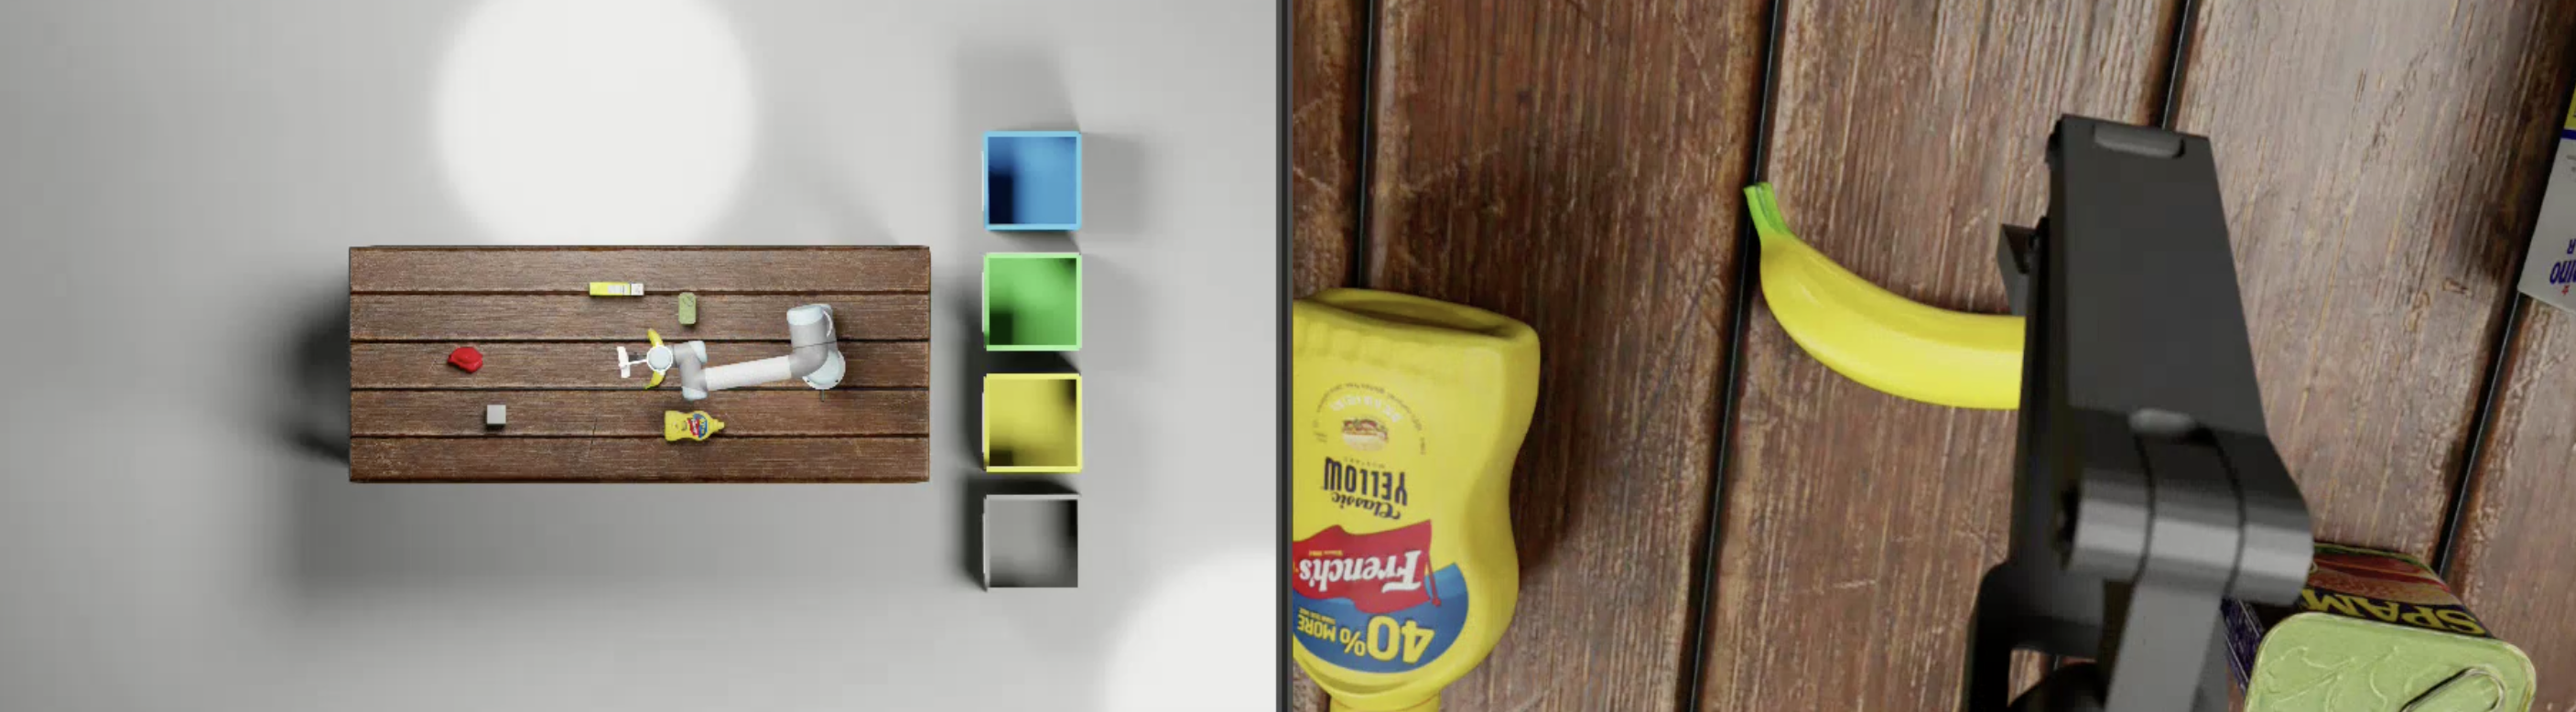
\includegraphics[width=\textwidth]{figures/fig_exp_setup1.png}
        \caption{Waste sorting domain overview. }
        \label{fig:dom1}
    \end{subfigure}
    \quad
    \begin{subfigure}[b]{0.47\textwidth}
        \captionsetup{skip=0pt}
	    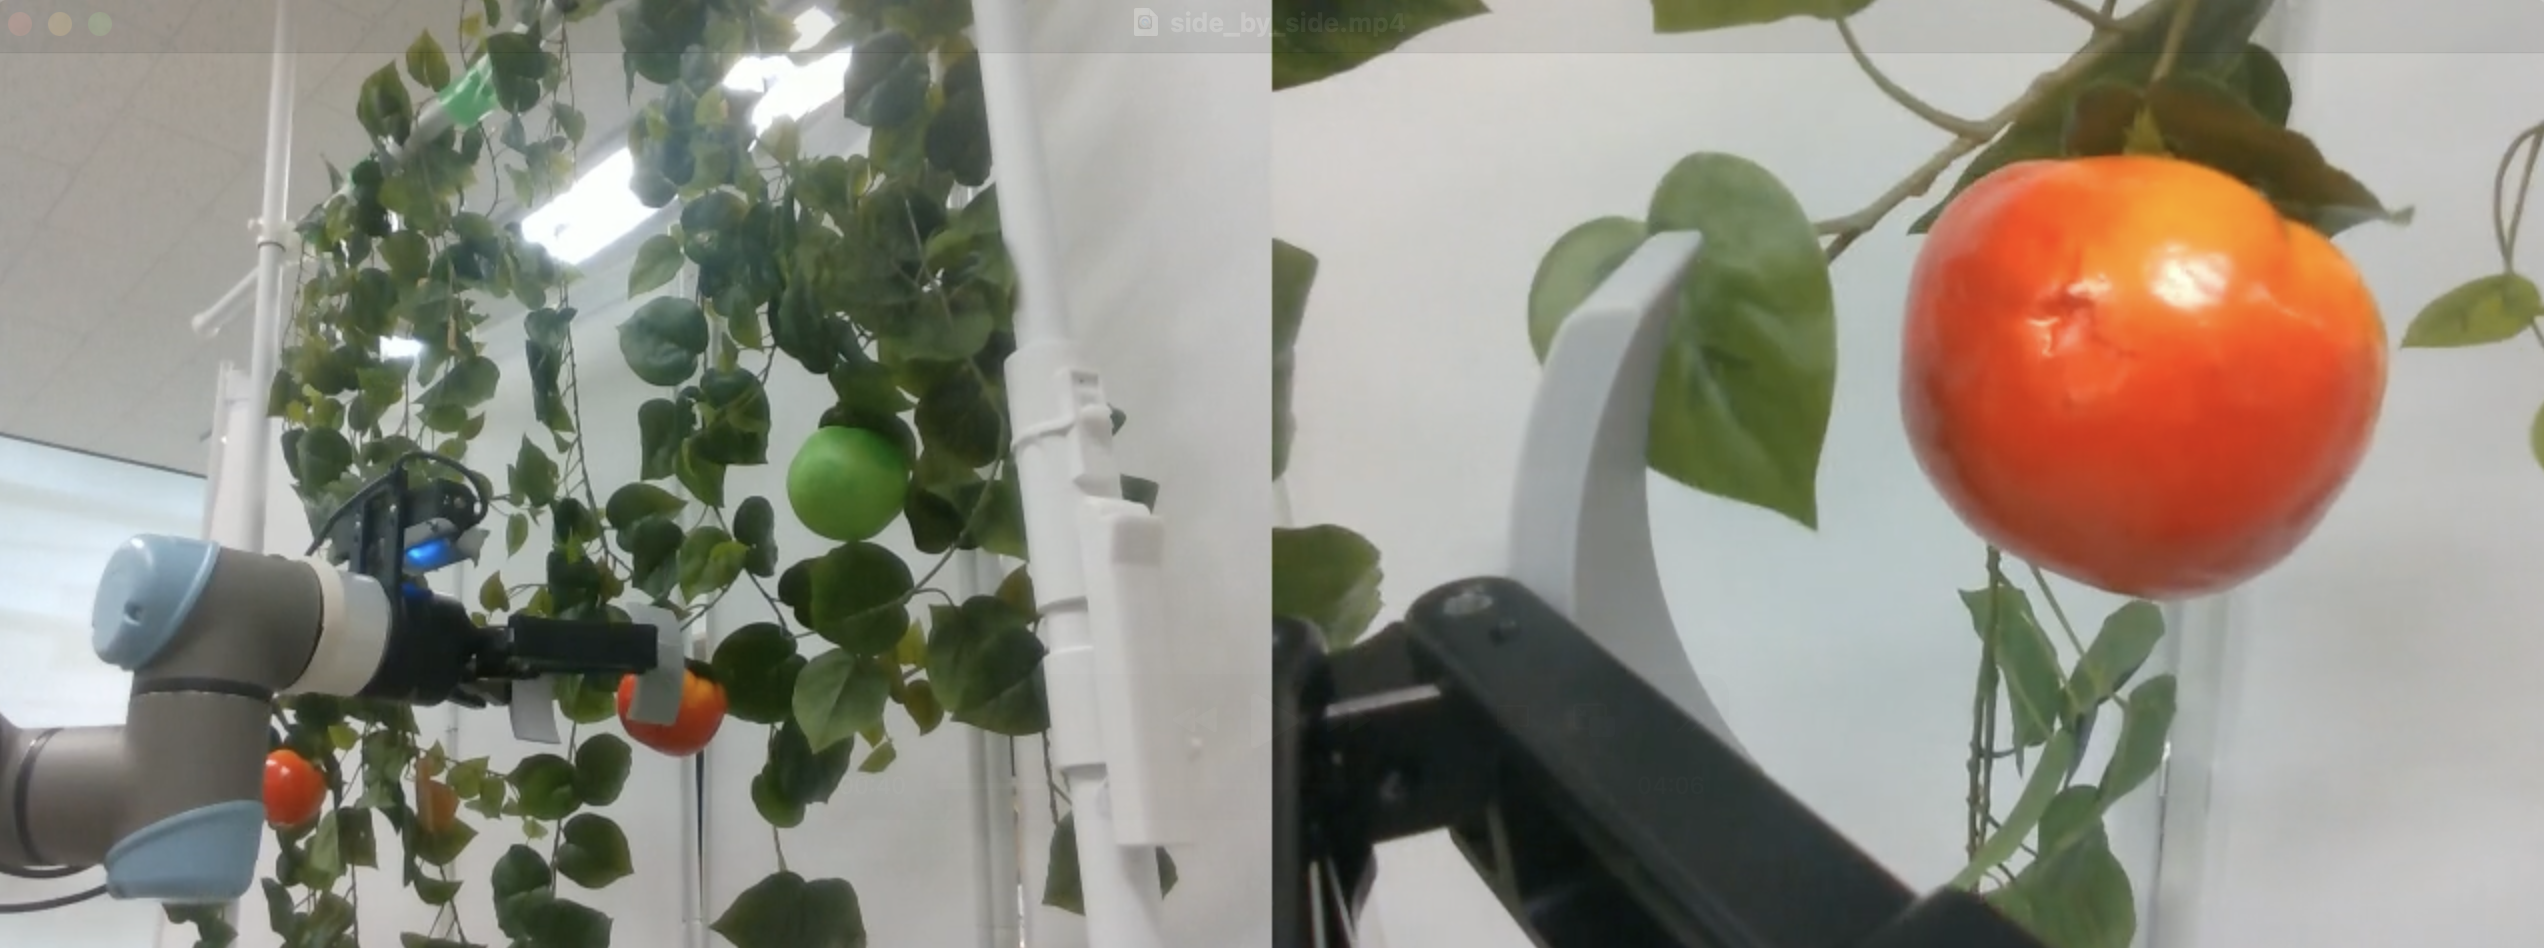
\includegraphics[width=\textwidth]{figures/fig_exp_setup2.png}
        \caption{Tomato harvesting domain overview}
        \label{fig:dom2}
    \end{subfigure}
    \caption{The illustration of the environments. (a) A UR5 robot sorts four types of waste into designated bins in Isaac Sim. (b) A mobile manipulator harvests ripe tomatoes and discards rotten ones in a real-world setting.}
  \label{fig:env_setting}
  
  \end{center}
\end{figure}


\subsection{Experimental Setup}~\label{exp:setup}
We evaluate the proposed method in two domains: a simulated waste sorting domain and a real-world tomato harvesting domain. The waste sorting domain is implemented in simulation using NVIDIA Isaac Sim, where a fixed UR5 robotic arm is used for pick and place task. Object detection is performed using the YOLOv12 model~\cite{tian2025yolov12}. In contrast, the tomato harvesting domain is deployed on a real mobile manipulator consisting of a UR5e robotic arm mounted on a Summit mobile platform. The robot is equipped with an RGB-D camera for visual perception and a LiDAR sensor for localization, and performs object detection using the same YOLOv12. 


\subsubsection{Waste sorting domain}~\label{exp:setup_waste}
We consider a tabletop waste-sorting scenario with four waste objects placed on a table, as shown in Fig.~\ref{fig:dom1}. A fixed UR5 robot is positioned between the objects and the recycling bins and performs three actions: \texttt{detect}, \texttt{pick}, and \texttt{place}. We assume that all objects are reachable by the manipulator.

Each object belongs to one of four categories: \texttt{general}, \texttt{paper}, \texttt{can}, and \texttt{plastic}. The object categories are not known a priori and must be inferred through perception. Since objects may be partially occluded by others, a single observation may not reveal all categories, requiring repeated detection during execution. The \texttt{detect} action can observe multiple objects simultaneously, after which the robot places each object into the corresponding recycling bin.

The initial arrangement of objects is randomized in every episode. A task is considered successful when all objects are correctly sorted within the maximum step limit. A reward of $+5$ is assigned when a waste object is placed into the recycling bin corresponding to its category, and an additional reward of $+10$ is given when all objects are correctly sorted. All other actions receive zero reward.



\subsubsection{Tomato harvesting domain}~\label{exp:setup_tomato}
We consider a tomato harvesting scenario in which four tomatoes are attached to two stems, denoted as \texttt{stem\_1} and \texttt{stem\_2}, as shown in Fig.~\ref{fig:dom2}. The robot navigates between three locations: \texttt{dock\_station}, \texttt{stem\_1}, and \texttt{stem\_2}, and performs \texttt{detect}, \texttt{pick}, \texttt{scan}, \texttt{place}, and \texttt{discard} actions.

Each tomato can be in one of three states: \texttt{ripe}, \texttt{unripe}, or \texttt{rotten}. The tomato states are initially unknown and must be estimated through perception. During detection, ripe and rotten tomatoes are visually ambiguous and cannot always be reliably distinguished. To resolve this ambiguity, the robot performs a \texttt{scan} action after picking a tomato to verify its condition before harvesting or discarding it. Unripe tomatoes are left untouched.

The tomato locations are randomized across stems in every episode. A task is considered successful when all ripe tomatoes are harvested and all rotten tomatoes are discarded within the maximum step limit. A reward of $+5$ is assigned when a ripe tomato is correctly harvested or a rotten tomato is correctly discarded after scanning. An additional reward of $+10$ is given when all task-relevant tomatoes are processed correctly. All other actions receive zero reward.



\subsubsection{Implementation Details}~\label{exp:details}
In all experiments, the planner used a discount factor $\gamma=0.95$, UCB exploration constant $c=1.0$, maximum simulation depth $depth_{\max}=20$, and $\Timeout=100$ Monte Carlo simulations per planning step. Each episode was limited to $50$ steps. For the policy comparison experiment, the confidence threshold for triggering user feedback was set to $\tau=0.8$ based on the threshold sweep reported in Sec.~\ref{exp:sys_eval}.

% \subsubsection{Evaluation Metrics}~\label{exp:metrics}
% \cp{We evaluate the proposed method based on task performance and human workload. Task performance is quantified using the task success rate, defined as the percentage of episodes in which the robot reaches the goal state required by each domain within maximum steps. An episode is considered a failure if the planner reaches a dead-end state or exceeds the maximum step limit. To assess the efficiency of human intervention, we additionally report the query frequency, measured as the average number of queries per episode. For the user studies, we employ the NASA-TLX questionnaire to evaluate subjective workload. Furthermore, we compare our state-level querying strategy with the KnowNo framework, which queries action-level decisions, to analyze their respective impacts on user workload and task success.}
